\section{Établir un modèle de données}
    \subsection{Réalisation d'un échantillon des données}

La préparation des données du projet \COREL s'effectue en coopération avec le prestataire. En effet, la société Data Futures est le gestionnaire de la plateforme d'annotation dans laquelle les chercheurs saisissent les données manquantes pour le projet, notamment les dates de début de période d'application des lois et les liens d'association et/ou d'association dirigée entre les lois. Ces informations sont présentes dans les annotations mais ont besoin d'être explicitées afin de pouvoir être ajoutées dans l'encodage : il est nécessaire d'ajouter des dates de fin d'application des lois notamment. L'équipe du projet a donc fait appel au prestataire afin de générer automatiquement les dates de fin de validité des lois à partir des liens de généalogie. Lorsqu'une loi en remplace une autre, la date de promulgation de la nouvelle loi marque la fin de l'application de la précédente. La chaîne de traitement des données est donc la suivante : les chercheurs enrichissent les données des annotations et les corrigent ; le prestataire génère automatiquement les dates de fin de validité des lois pour obtenir des bornes chronologiques ; les données sont ajoutées à l'encodage \TEI. Lors du stage, la première étape de cette chaîne de traitement était en cours de réalisation. La deuxième étape, prévue dans le calendrier du projet, indique que le prestataire fournit les données via des fichiers \JSON au mois de septembre. 

Afin d'anticiper la dernière étape de préparation des données, un échantillon des données a été réalisé sur un extrait du \dc, chapitre 6, section 25, \lu 254 et \li 1. Cet échantillon permet d'encoder les données manquantes afin d'établir le modèle d'encodage qui sera utilisé pour ajouter les données \JSON en \TEI. Dans un premier temps, il a été nécessaire d'identifier tous les types de données à ajouter et de déterminer les éléments \TEI les plus pertinents pour encoder ces informations. Cette étape a été réalisée une fois les documents \XML transformés en \TEI. Pour mener à bien le projet, il est pertinent d'ajouter dans l'encodage : 
\begin{itemize}
    \item Les bornes chronologiques pour chaque \lu et \li.
    \item Le lien vers les numérisations des textes.
    %à vérifier : est-ce que j'ai parlé au début du fait qu'on veut inclure les numérisations dans le site web, dans un visualiseur 3IF ?? mais que les ressources ne sont pas accessibles en ligne et que on ne peut pas accéder aux manifestes ? (et que l'équipe du projet ne le souhaite pas ?????)
    \item Un identifiant unique pour chaque \lu et \li permettant d'identifier dans chaque texte les lois associées.
    \item Des commentaires supplémentaires (de nature différente des commentaires officiels).
    \item L'enrichissement des données sur les entités nommées.
\end{itemize}

Ces éléments ont été choisis conjointement avec les chercheurs afin d'obtenir en résultat une édition en ligne complète et exploitable pour les chercheurs. À partir de cette liste, un modèle d'encodage à suivre a pu être mis en place. 

\begin{minted}{xml}
    <div type="substatute" n="1" xml:id="DQLL_254_1" 
         notBefore="1833" notAfter="1870">
        <pb  
        facs="https://duli-cunyi.freizo.org/mirador/book.cgi?catno=28941&amp;
        canvas=https://iiif.duli-cunyi.freizo.org/image/28941/canvas/p5"/>
            <p>一、反逆案内律應問擬凌遲之犯,其子孫訊明,
            實係不知謀逆情事者,無論已未成丁,均解交内務府閹割,發往新疆等處,
            給官兵為奴。如年在十歲以下者,牢固監禁,俟年届十一歲時,再行解交内務府,
            照例辦理。内務府大臣遇有解到閹割人犯,即遴派司員認眞看驗,並出具無弊切結,
            送交刑部,再行覆驗。如有情弊,即行奏參,務須查驗明確,再交兵部,發往新疆,
            給官兵為奴。至其餘律應緣坐男犯,並非逆犯子孫,年在十六歲以上者,
            發往新疆等處,給官兵為奴。如年在十五歲以下者,牢固監禁,
            俟成丁時再行發遣。緣坐婦女,發各省駐防,給官員兵丁為奴。
            其知情不首干連人犯,仍依律擬流。</p>
            <note type='metadata'>Notes on the law</note>
    </div>
\end{minted}

\subsubsection{Liens vers les images}
Les liens vers les images peuvent être ajoutés via l'attribut \texttt{@facs} sur les balises \texttt{<pb/>} qui indiquent le début d'une nouvelle page. Ces balises ont été ajoutées aux sources numériques afin de faciliter la pagination de l'édition numérique et permettra d'afficher l'image en regard du texte. Le projet \COREL souhaite aboutir à une éditon simple qui propose le texte et l'image correspondante à la page près. Un facsimile interactif n'est pas envisagé, c'est pourquoi seul l'attribut \texttt{@facs} a été choisi pour intégrer les images à l'encodage. Cette solution a également été adoptée pour le projet \cordel : 
\begin{minted}{xml}
     <div>
        <pb n="1" source="Moreno_001_1.jpg" 
        facs="fedora_ug8110021/full/full/0/default.jpg"/>
\end{minted}

L'intégration des images pose toutefois un problème d'\textit{open access} qui n'a pas pu être résolu dans le cadre de mon stage. En effet, l'équipe du projet ne dispose pas des liens \IIIF des images, contrairement au projet \cordel. Une \URL \IIIF accepte plusieurs paramètres qui permettent d'afficher différentes zones de l'image à partir des pixels. Dans l'exemple du projet \cordel, l'image est affichée en entier grâce au paramètre \texttt{full}. \footnote{Ressource image issue de l'article \og C'est quoi le IIIF ? \fg de l'Université de Genève.} Les liens \IIIF des numérisations des codes légaux, de même que les liens des ressources images seules (indiquées dans les fichiers \JSON en tant qu'identifiant), ne sont pas disponibles sur le web. Le prestataire ne fournit que le lien permettant d'accéder à l'image via leur serveur. Cela pose un problème d'accessibilité, en cours de résolution par l'équipe du projet, afin que les numérisations soient librement accessibles sur le web et que les liens puissent être inclus dans l'édition numérique. Dans l'échantillon, il a été décidé d'inclure le lien présent dans les fichiers \JSON, bien qu'il ne soit pas accessible pour le moment. Une fois l'accès autorisé par le prestataire, utiliser les liens des fichiers \JSON permettra d'automatiser l'ajout des liens dans l'encodage via un script. Cette solution est la plus satisfaisante pour le projet, étant donné que la majorité des informations à ajouter doivent l'être depuis les fichiers \JSON. 

\begin{figure}
    \centering
    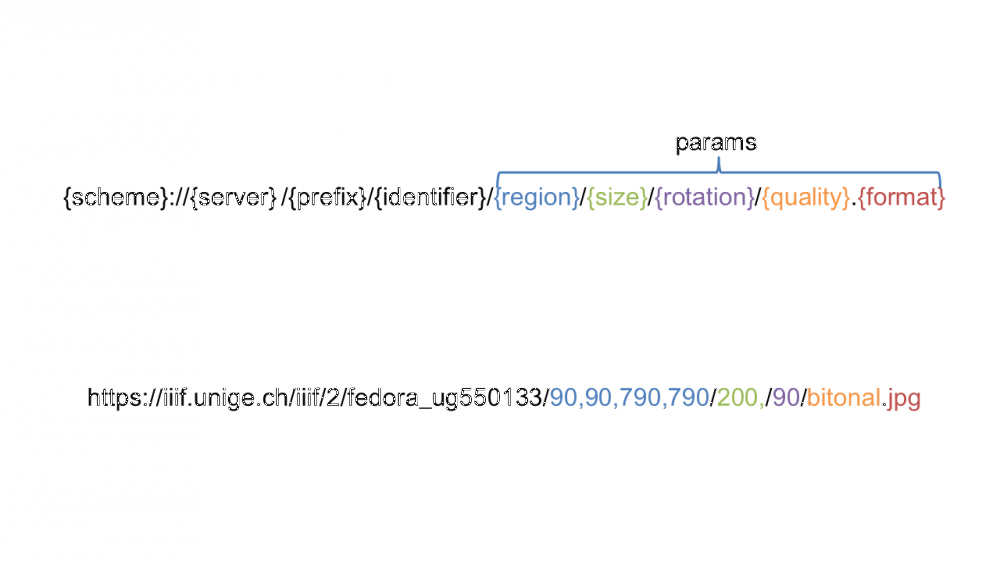
\includegraphics[width=\textwidth]{images/iiif.png}
    \caption{Schéma explicatif d'une \URL \IIIF}
\end{figure}

\subsubsection{Les bornes chronologiques et les identifiants \XML}
L'ajout des bornes chronologiques est également permis par des attributs \TEI. Sur chaque \lu et \li, contenues dans des éléments \texttt{<div>}, il est possible d'ajouter des attributs \texttt{@notBefore} et \texttt{@notAfter} afin d'ajouter les dates à l'encodage. Toutefois, cet ajout demande un élargissement des règles de la \TEI car ces attributs ne sont pas autorisés sur des éléments \texttt{<div>}. L'ajout de ces attributs est indispensable afin de reconstituer la législation pour une année donnée. Placer ces attributs sur les balises \texttt{<div>} est nécessaire afin de pouvoir afficher la loi contenue dans cette balise afin de créer le \cv, c'est pourquoi la modification de la \TEI a été choisie pour cet élément. En plus de ces bornes chronologiques, l'élément \texttt{<div>} contient l'attribut \texttt{@xml:id} qui permet d'attribuer à chaque loi un identifiant unique. Cela permet de faire le lien avec les fichiers \JSON et d'attribuer aux lois associées, c'est-à-dire les lois qui sont les mêmes d'un texte à un autre, le même identifiant. 

Les données à inclure dans les attributs font le lien entre le format \XML et le format \JSON. Toutefois, d'autres informations d'enrichissement des données doivent être ajoutées. 

\subsubsection{Les commentaires et les entités nommées}
Les commentaires et les entités nommées sont des informations additionnelles, qui ne sont pas présentes dans les annotations. En effet, les commentaires ont été océrisés mais n'ont pas été ajoutés dans l'encodage \XML du projet \LSC, ni dans les annotations. Quelques informations sur les entités nommées ont été ajoutées dans les annotations, toutefois elles restent partielles et n'ont pas été corrigées. 

Plusieurs types de commentaires existent dans les textes de lois chinois. Les commentaires officiels, rédigés en même temps que le texte de loi, sont déjà présents dans l'encodage dans des éléments \texttt{<note type='official'>}. Ils apparaissent dans les sources originales dans une police de caractère légèrement inférieure. Sur le site web \LSC, l'affichage met en valeur ces commentaires avec une couleur différente du reste du texte. D'autres commentaires, notamment d'auteurs ayant rédigés les compilations, seront ajoutés à l'édition en ligne. Elles sont représentées dans l'échantillon par des balises \texttt{<note>}, toutefois leur type n'a pas encore été défini. À des fins explicatives, un attribut \texttt{@type} a été ajoutés sur ces balises pour indiquer que chaque commentaire doit posséder cet attribut obligatoire, avec un type défini.

De plus, des commentaires qui ne sont pas présents dans l'\OCR peuvent également être ajoutés, afin de créer dans l'édition en ligne un mode \og métadonnées \fg qui permettrait d'afficher des informations supplémentaires sur les lois. Ces commentaires ont donc un attribut \texttt{@type='metadata'}. 

Par ailleurs, l'équipe du projet souhaite également enrichir les informations sur les entités nommées, afin d'envisager dans l'édition en ligne un mode \og entités nommées \fg pour les mettre en avant. Dans l'encodage \LSC, les entités nommées sont balisées par des éléments \texttt{<personname>} ou \texttt{<propername>}. Le projet \COREL souhaite encoder un peu plus précisément les noms de personnes en leur ajoutant notamment un nom de rôle : 

\begin{minted}{xml}
    <persName role="governor" ref="#覺羅伍拉納">
        <roleName>福建巡撫</roleName>
        <name>覺羅伍拉納</name>
    </persName>
\end{minted}
En effet, la plupart des personnes mentionnées sont des fonctionnaires et ont donc un rôle qui peut être mis en valeur dans l'encodage. Afin d'éviter les erreurs d'encodage et de garantir sa régularité, il est pertinent d'ajouter dans le \texttt{<teiHeader>} les informations relatives à ces entités nommées dans un élément \texttt{<listPerson>} : 

\begin{minted}{xml}
     <listPerson>
        <person xml:id="覺羅伍拉納">
            <persName role="governor" ref="#覺羅伍拉納">
                <roleName>福建巡撫</roleName>
                <name>覺羅伍拉納</name>
            </persName>
            <note>Biographical information</note>
        </person>
        <person xml:id="何東山">
            <persName role="party" ref="#何東山">
                     何東山
            </persName>
            <note>Biographical information</note>
        </person>
        <person xml:id="何適">
            <persName role="party" ref="#何適">
                     何適
            </persName>
            <note>Biographical information</note>
        </person>
    </listPerson>
\end{minted}
Lister les entités nommées dans le \texttt{<teiHeader>} permet de les identifier grâce à un attribut \textit{@xml:id} et donc d'afficher les informations relatives à chaque entité nommée si un mode \og entités nommées \fg est créé pour le site web. Le lien entre l'identifiant \XML et le nom de personne dans l'encodage s'effectue grâce à l'attribut \texttt{ref.} Le modèle d'encodage des entités nommées a pu être déterminé grâce à l'exemple du projet \disco de l'INRIA. En effet, leur projet accorde une place importante aux entités nommées puisqu'ils offrent une édition numérique de correspondances : 
\begin{minted}{xml}
     <listPerson>
        <person xml:id="p0001">
            <persName>d'Estournelles de Constant, Paul</persName>
            <persName>
                <roleName type="nobility">Baron</roleName>
                <forename>Paul</forename>
                <nameLink>d'</nameLink>
                <surname>Estournelles de Constant</surname>
            </persName>
            <persName>Paul Henri Balluet d'Estournelles de Constant</persName>
            <nationality>French</nationality>
            <birth>
                <date when-iso="1852-11-22"/>
                <placeName>La Flèche (Sarthe)</placeName>
            </birth>
            ...
        </person>
    </listPerson>
\end{minted}
L'édition en ligne de \disco offre un encodage exhaustif des entités nommées, dans un fichier d'index \TEI dédié à cet usage. Dans le cadre du projet \COREL, un fichier d'index n'est pas envisagé pour le moment étant donné que le corpus est constitué d'un nombre restreint de documents et que les entités nommées ne sont pas le centre du projet. Toutefois, la liste des entités nommées pourra être transposée dans un index si l'encodage s'enrichit et donne lieu à une liste et à des informations exhaustives. Pour ajouter des informations additionnelles pour chaque entité nommée, l'échantillon propose une balise \texttt{<note>} pour ajouter des informations biographiques, sans structure prédéfinie, qui pourront être affichées dans le mode \og entités nommées \fg. 

Pour le balisage des noms de lieux, une structure similaire a été mise en place dans l'échantillon. Une liste des lieux est présente dans le \texttt{<teiHeader>} : 
\begin{minted}{xml}
     <listPlace>
        <place xml:id="寧古塔">
            <placeName ref="#寧古塔">
                寧古塔
            </placeName>
            <note>Information about the place</note>
        </place>
    </listPlace>
\end{minted}
À l'instar des noms de personnes, le nom du lieu possède un identifiant unique qui permet de le lier au balisage présent au sein du texte et un élément \texttt{<note>} afin d'ajouter des informations supplémentaires sur le lieu. Les noms de lieux sont mentionnés dans les textes de loi en tant que lieu d'où provient l'origine de la loi ou bien en tant que lieu d'application. Selon le contexte, la balise \texttt{<placeName>} porte donc l'attribut \texttt{@type} avec pour valeur \texttt{'application'} ou \texttt{'origin'}. 

L'établissement d'un échantillon des données permet ainsi de fournir un modèle d'encodage à suivre pour la suite du projet et donne un aperçu de l'état final du jeu de données \TEI. L'exercice a pu mettre en valeur les difficultés qui peuvent être rencontrées lors de l'encodage, notamment l'accessibilité des ressources ou le besoin d'étendre la \TEI, et ainsi de les anticiper et de commencer à les résoudre en amont afin de pouvoir enrichir le jeu de données dès le mois de septembre. Toutefois, il est également pertinent d'étudier les limites de cet aperçu idéalisé des données.

\subsection{Limites de cet aperçu idéalisé des données}
L'échantillon de données offre un modèle de données à suivre afin de réaliser le projet. Toutefois, il représente un aperçu idéalisé des données telles que l'équipe du projet les envisage à la fin du financement, afin d'offrir aux chercheurs une édition scientifique numérique la plus complète possible. Les contraintes de temps et de financement peuvent influer sur ce modèle de données et son niveau de complétude. L'échantillon permet alors de mettre en lumière les informations manquantes dans l'encodage à un instant T, notamment les informations qui seront essentiels pour mener à bien le projet (les bornes chronologiques et les identifiants \XML notamment). Cet aperçu idéalisé des données peut être réalisé dans le périmètre du projet en automatisant l'encodage via des scripts : les données à ajouter depuis les fichiers \JSON pourront être ajoutées automatiquement. Cependant, le balisage des entités nommées et l'ajout des commentaires sont des données disponibles en texte brut sans balisage, ce qui nécessite un travail supplémentaire de la part de l'équipe du projet. L'encodage des commentaires est actuellement en cours de traitement, mais dans le modèle de données du projet \LSC. Une étape supplémentaire de transformation devra donc être prise en charge par le projet. Cet enrichissement des données \LSC est hors périmètre du projet \COREL. Cependant, les chercheurs continuent d'alimenter les projets antérieurs, ce qui ajoute une étape supplémentaire dans le traitement des données. Les commentaires encodés en \XML devront être transformés en \TEI via \XSLT ou via un script. 

De plus, le travail sur les entités nommées est également en cours de traitement. Les rôles des fonctionnaires commencent à être identifiés dans les annotations, mais ces informations, repérées et ajoutées une à une par les chercheurs à la lecture des textes de loi, demande un travail de recherche long et exhaustif. Lors du stage, il a été envisagé d'utiliser un outil d'encodage automatique en \TEI, MARKUS. MARKUS est un outil qui permet de reconnaître les entités nommées (noms de personnes, de lieux et dates notamment) pour les textes chinois et coréens. C'est un outil open source, accessible en ligne qui prend en entrée du texte brut et place des balises \TEI uniquement sur les entités nommées. Un test avec l'un des documents du corpus a été réalisé afin d'envisager un traitement automatique de l'encodage. MARKUS, cependant, est une version bêta en cours de production. Bien qu'il balise les entités nommées, les documents \TEI obtenus en sortie ne sont pas valides car seules les entités nommées sont balisées, sans racine \texttt{<TEI>} et autres balises obligatoires. Puisque les sources numériques devaient être transformées en \TEI afin de proposer une édition en ligne, l'équipe du projet a donc envisagé d'ajouter aux documents \TEI finaux les informations supplémentaires obtenues par MARKUS via un script. Cependant, à l'analyse des résultats fournis, la reconnaissance d'entités nommées contenait trop peu d'informations exactes pour justifier cette étape supplémentaire dans le traitement des données : utiliser les balises de MARKUS demande plusieurs étapes supplémentaires dans la préparation des données : une phase de relecture des résultats, puis l'ajout des entités nommées dans le corpus \TEI et enfin la vérification du résultat final obtenu. Le travail de correction a été estimé trop important, car beaucoup de bruit était généré par le balisage automatique. Par exemple, certains noms étrangers sont retranscris en chinois par des chiffres. Une confusion entre des chiffres et des noms de personnes pouvait donc être constatées dans l'encodage automatique. Un autre exemple de balisage par MARKUS montre un mésusage des attributs \TEI : 

\begin{minted}{xml}
    <roleName n="officialTitle">法司</roleName>
\end{minted}

L'attribut \texttt{@n}, utilisé pour la numérotation, est souvent utilisée par MARKUS comme un attribut \texttt{@type}. Cette solution n'a donc pas été adoptée car l'échéance du projet ne permet pas un laps de temps suffisant pour utiliser au mieux cet outil. 

L'échantillon de données et ce travail de réflexion sur la manière d'enrichir les données du projet a été le moyen de déterminer quelles données sont primordiales afin de réaliser le projet et lesquelles sont un enrichissement pertinent à proposer aux chercheurs sans pour autant être des données décisives pour la bonne réalisation des livrables.
%peut être rajouter un exemple de code sorti par Markus

 \section{Un schéma d’encodage}
    \subsection{La documentation de l’encodage}

En prenant appui sur le jeu de données \TEI de référence établi pendant le stage et sur l'échantillon des données, il a été possible de mettre en place une \ODD afin de documenter les sources du projet et de mettre en place un schéma d'encodage à suivre. 

Les projets d'édition scientifique numérique s'accompagnent en effet d'une documentation en prose dans l'\ODD. Cette documentation ne remplace pas les \textit{guidelines} de la \TEI mais viennent les compléter afin d'expliciter les spécifités d'encodage du corpus, la structure des documents et les choix faits par l'équipe. Cela est utile à la fois à l'équipe, qui peut se référer à des documents de travail clairs et aux utilisateurs qui consulteront les données une fois publiées. 

L'\ODD a été rédigée selon le modèle de données final que le projet souhaite obtenir. Certains éléments ne sont donc pas encore présent dans le jeu de données \TEI mais figurent dans l'échantillon à titre d'exemple. L'\ODD reste modifiable par l'équipe du projet si les choix d'encodage venaient à changer lors de la préparation des données tout en offrant un guide d'encodage précis à suivre agrémenté d'exemples tirés du corpus ou de l'échantillon : 

\begin{minted}{xml}
    <div>
        <head>
            <gi>particDesc</gi>
        </head>
        <p>
            The <gi>particDesc</gi> element contains the list of 
           <gi>persName</gi> present in the code. 
           Each <gi>person</gi> is attributed 
            <ref target="ODD_COREL.html#TEI.person">
                a mandatory <att>xml:id</att>
            </ref> 
            and a 
            <ref target="ODD_COREL.html#TEI.person">
                mandatory <att>role</att>.
            </ref> 
            Inside the <gi>person</gi> element, 
            the <gi>persName</gi> element must contain 
            <ref target="ODD_COREL.html#TEI.persName">
                the <att>ref</att>attribute.
            </ref> 
            Biographic notes about the person can be included if
                  necessary.
        </p>
        <egXML xmlns="http://www.tei-c.org/ns/Examples">
            <listPerson>
                <person xml:id="覺羅伍拉納">
                    <persName role="governor" ref="#覺羅伍拉納">
                        <roleName>福建巡撫</roleName>
                        <name>覺羅伍拉納</name>
                    </persName>
                    <note>Biographical information</note>
                </person>
                <person xml:id="何東山">
                    <persName role="party" ref="#何東山"> 何東山 </persName>
                    <note>Biographical information</note>
                </person>
            </listPerson>
        </egXML>
    </div>
\end{minted}

Chaque élément de l'encodage et l'utilisation qui en est faite sont décrits, avec la liste des éléments enfants lorsque l'élément peut contenir d'autres éléments \TEI. Les règles de validation spécifiques au corpus (le nombre de fois que l'élément apparaît, les attributs et/ou éléments obligatoires...) sont également définies. Un exemple permet ensuite d'illustrer la définition des éléments. 

L'\ODD rédigée a enfin été transformée via le scénario de transformation \textit{oddbyexample}. Ce schéma de transformation permet d'obtenir un fichier \HTML afin d'accéder au guide d'encodage.

\begin{figure}
    \centering
    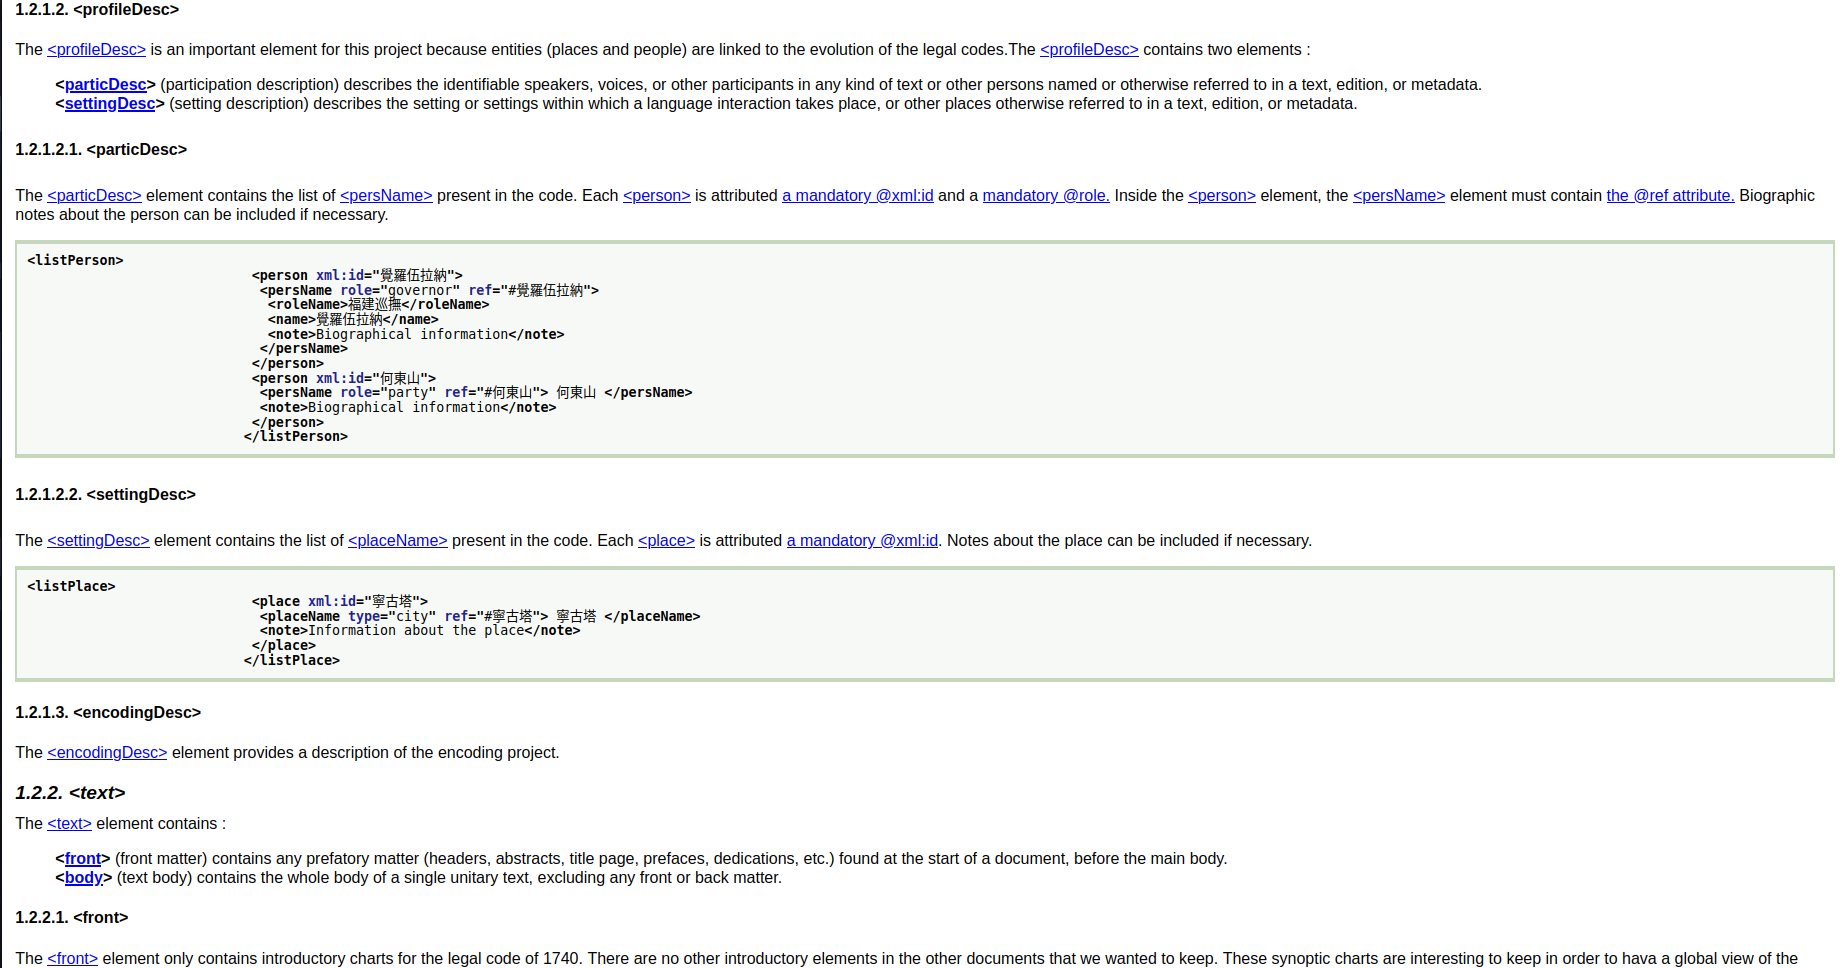
\includegraphics[width=\textwidth]{images/odd.png}
    \caption{Capture d'écran du guide d'encodage en \HTML}
\end{figure}

La page \HTML de sortie présente un sommaire puis la documentation rédigée ainsi que les règles de validation du document \TEI. Une mise en page similaire à celle des \textit{guidelines} est obtenue. Des liens hypertextes permettent de naviguer dans le guide depuis la table des matières, vers la documentation en prose et les règles de validation, retranscrites sous forme de tableau comme dans les \textit{guidelines}.

\begin{figure}
    \centering
    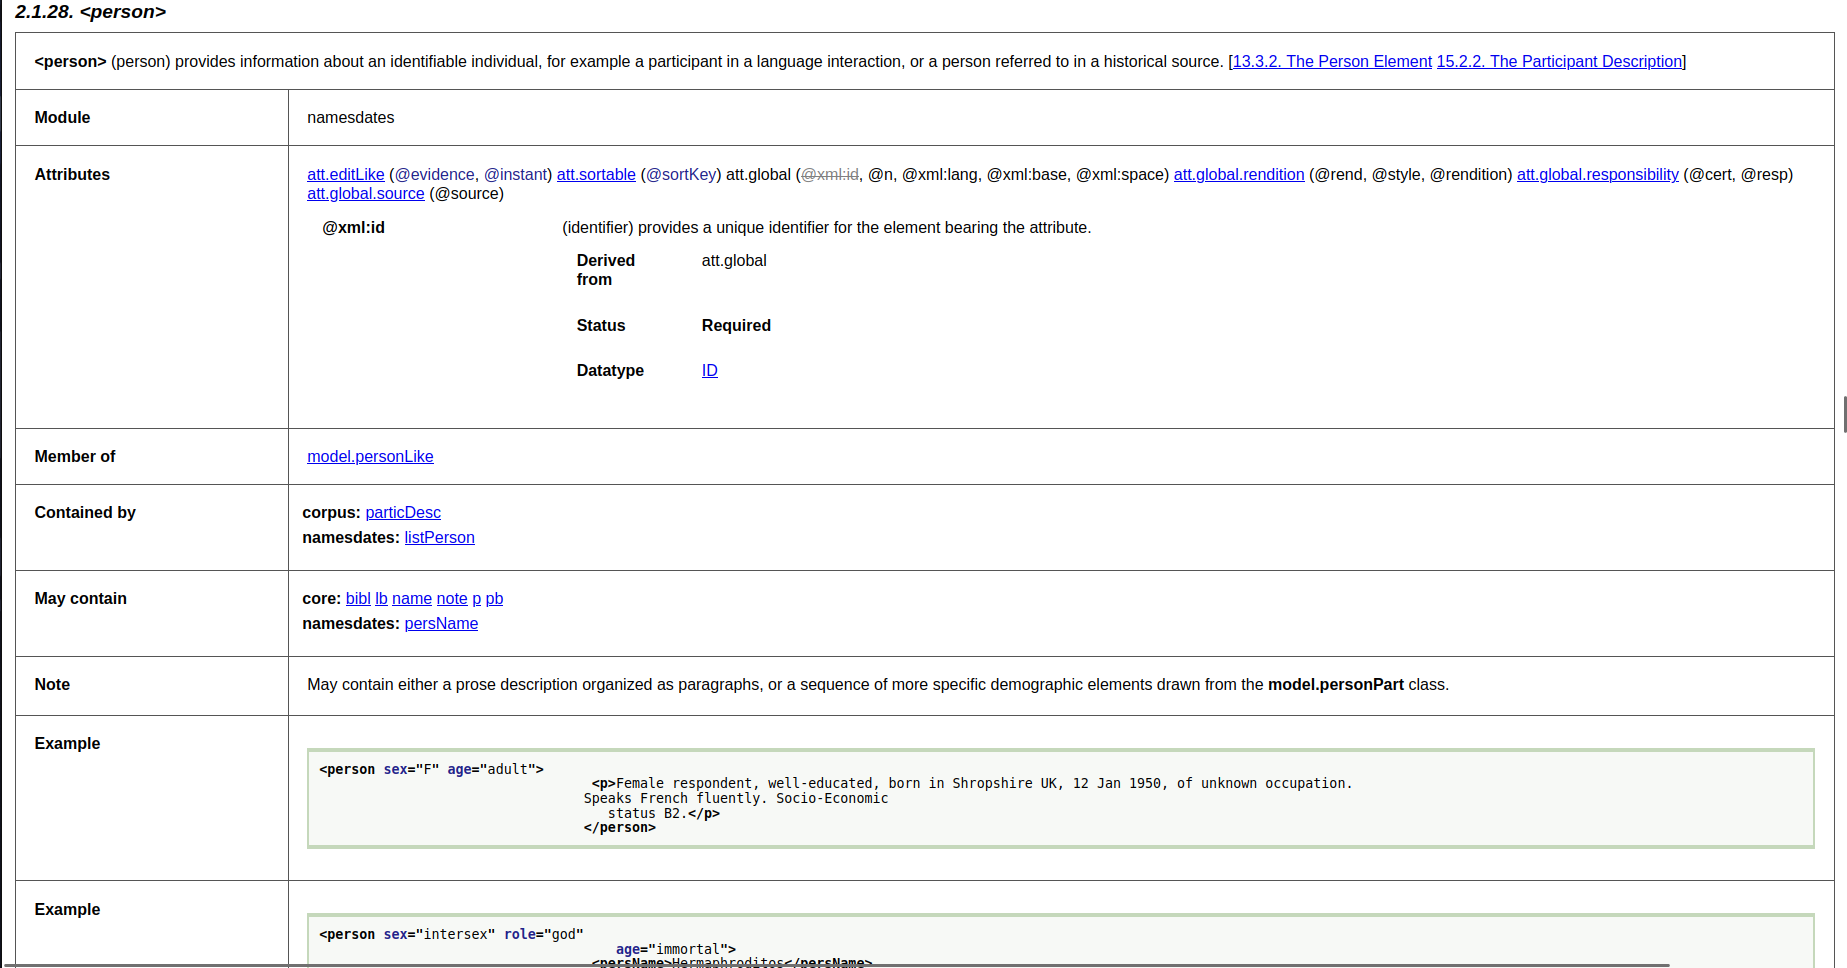
\includegraphics[width=\textwidth]{images/odd2.png}
    \caption{Capture d'écran des règles de validation en \HTML}
\end{figure}

Le scénario \textit{oddbyexample} fournit également en sortie un fichier \RNG afin de le lier aux documents \TEI pour mettre en place un schéma de validation.

\newpage
\subsection{Le schéma de validation}

L'\ODD permet également de rédiger des règles de validation afin de faciliter l'encodage en \TEI et de mettre en lumière les informations manquantes ou mal encodées. En effet, la mise en place d'un schéma de validation permet, via le logiciel \textit{Oxygen}, de faire apparaître les erreurs via un code couleur : rouge pour les erreurs de première importance, et orange pour les manquements de l'encodage. 

Plusieurs règles d'encodage ont donc été définies à partir des documents du corpus ainsi que l'échantillon. Les textes de lois suivant une structure rigoureuse, les éléments \texttt{<div>} ont fait l'objet de règles strictes afin de garantir que les erreurs de structure ou d'imbrication des éléments soient repérées : 

\begin{minted}{xml}
    <!-- Il doit y avoit 7 chapitres -->
    <constraintSpec scheme="schematron" ident="sequence" xml:id="rule05">
        <constraint>
            <s:rule context="tei:body">
                <s:assert test="count(tei:div[@type='chapter'])=7"> 
                Il doit y avoir 7 chapitres dans le document. 
                </s:assert>
            </s:rule>
        </constraint>
    </constraintSpec>
\end{minted}

Afin de pouvoir rédiger des règles sur certains types d'éléments \texttt{<div>} uniquement, la syntaxe \textit{Schematron} a été utilisée. Les règles \textit{Schematron} permettent de donner dans l'attribut \texttt{@context} un chemin \xpath. Ainsi, la règle ci-dessus ne s'applique qu'aux éléments \texttt{<div>} directement contenues dans la balise \texttt{<body>}. Ces divisions qui correspondent aux chapitres des textes de loi sont obligatoirement au nombre de sept. La syntaxe \textit{Schematron} a ainsi permis d'indiquer que chaque chapitre doit contenir une ou plusieurs sections, devant elles-mêmes contenir des \lu. Les règles de validation garantissent que la structure des documents orignaux est bien respectée et régulière tout au long de l'encodage. Ces règles de validation sont essentielles afin de publier une édition scientifique numérique utilisable par les chercheurs, dans le respect de l'architecture des codes légaux chinois. 

Certains éléments, en revanche, sont spécifiques à notre projet d'édition et ne sont pas primordiaux afin de réaliser les livrables du projet, comme par exemple l'intégration des images en regard du texte. Ces éléments sont importants pour remplir les objectifs du projet puisqu'inclure la numérisation des codes légaux dans le site web fait partie du périmètre. Toutefois, il ne s'agit pas d'erreurs de même niveau qu'un problème de structuration des textes, c'est pourquoi deux niveaux d'erreurs ont été distingués : 

\begin{minted}{xml}
    <constraintSpec scheme="schematron" ident="facs" xml:id="rule08">
        <constraint>
            <s:rule context="tei:body//tei:pb">
                <s:assert test="@facs" role="WARN"> 
                    L'attribut facs est obligatoire 
                </s:assert>
            </s:rule>
        </constraint>
    </constraintSpec>
\end{minted}

Dans la règle ci-dessus, l'attribut \texttt{role} permet de spécifier que la règle concernant l'ajout de l'attribut \texttt{@facs} pour l'intégration des images est obligatoire mais que le niveau d'erreur est inférieur à la règle précédente. La règle a donc un rôle d'\og avertissement \fg. Dans l'éditeur \textit{Oxygen}, elle apparaît en orange afin de la distinguer des erreurs de niveau supérieur.
 \begin{figure}
     \centering
     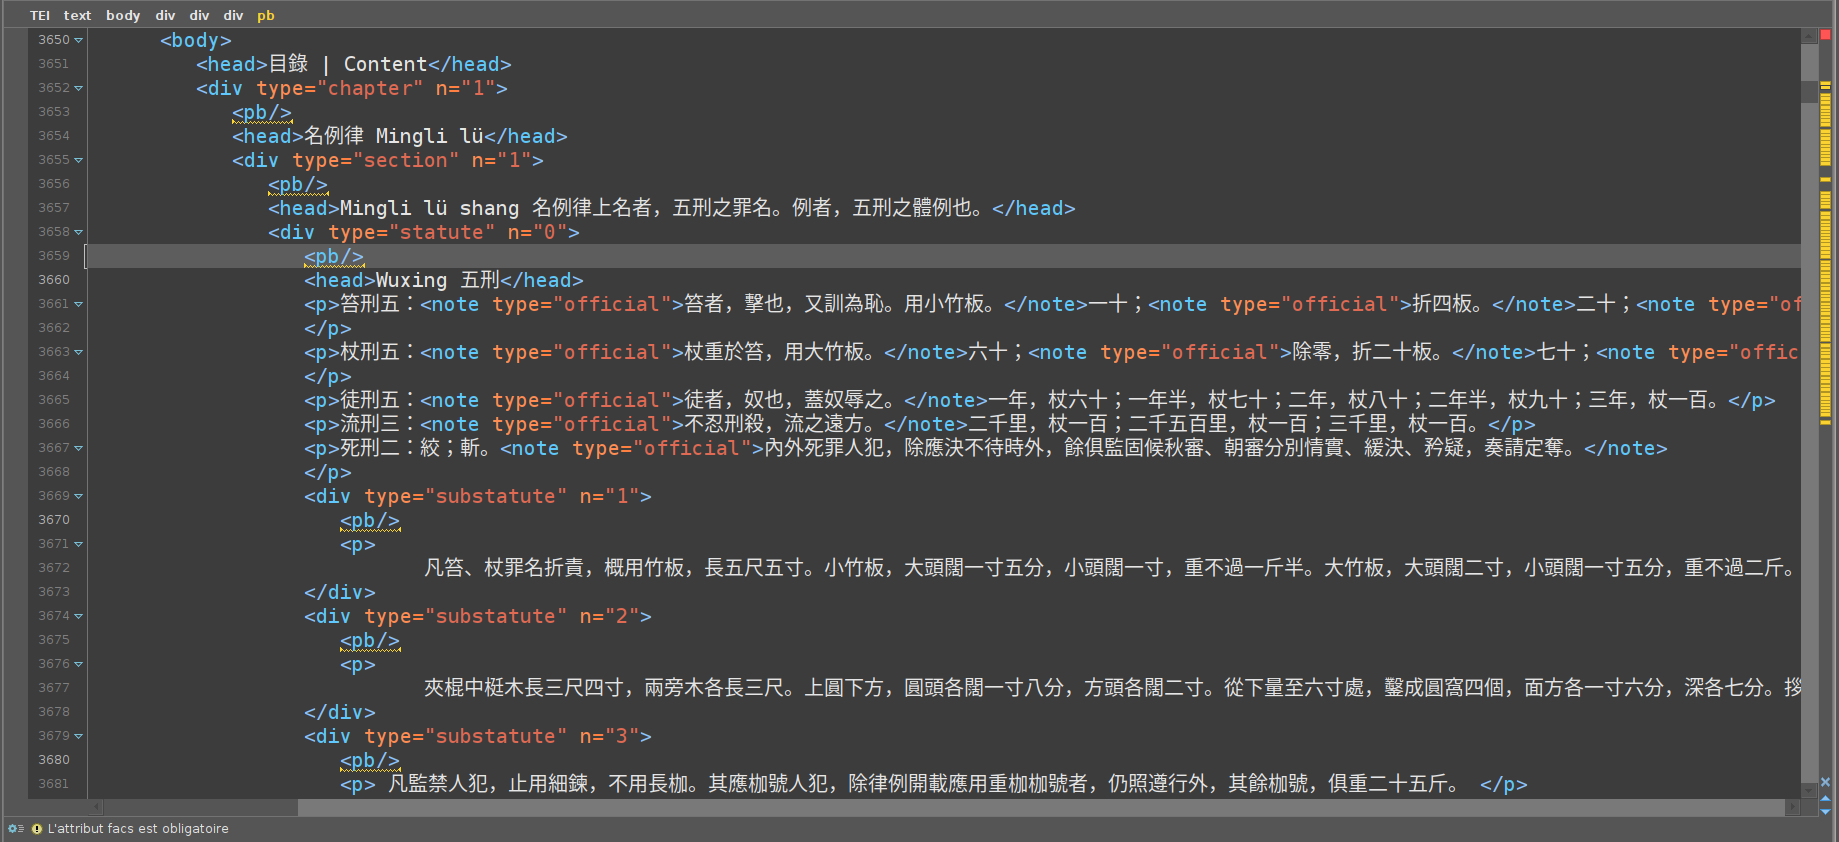
\includegraphics[width=\textwidth]{images/oxygen.png}
     \caption{Capture d'écran de l'affichage des erreurs sur Oxygen}
 \end{figure}

 \newpage
 C'est également dans l'\ODD qu'il est possible de modifier les règles de validation afin d'étendre la \TEI. Dans le cadre de la création d'un code légal généré automatiquement pour chaque année de la dynastie Qing, il est nécessaire d'encoder des périodes de validité pour chaque \lu et \li. Les attributs \texttt{@notBefore} et \texttt{@notAfter} ne sont pas autorisés sur les éléments \texttt{<div>}. La rédaction des règles de validation a donc permis d'ajouter ces attributs sur les divisions souhaitées. Pour cela, les attributs ont été ajoutés dans la liste des attributs autorisés sur l'élément \texttt{<div>} : 

 \begin{minted}
    <attList>
        <attDef ident="notBefore" mode="add"/>
        <attDef ident="notAfter" mode="add"/>
    </attList>
 \end{minted}

En plus de cet ajout, une règle \textit{Schematron} a été rédigée afin de spécifier que ces attributs sont obligatoires sur les \lu et les \li. 

Une fois le schéma d'encodage défini et les règles rédigées, la transformation via le scénario \textit{oddbyexample} a créé un fichier \RNG qui doit être lié aux documents \TEI comme ceci : 

\begin{minted}{xml}
<?xml-model href="ODD_COREL.rng" type="application/xml" \\ schematypens="http://relaxng.org/ns/structure/1.0"?>
<?xml-model href="ODD_COREL.rng" type="application/xml" \\ schematypens="http://purl.oclc.org/dsdl/schematron"?>
\end{minted}

L'éditeur \textit{Oxygen} prend ensuite en compte le schéma d'encodage défini et permet de souligner les erreurs selon les différents niveaux. Ces règles de validation sont essentielles afin de permettre à l'équipe du projet de poursuivre l'encodage et atteindre le modèle de données souhaitées. La création de règles de validation permet de mettre en avant les données manquantes dans les documents et de guider l'ajout des données, ce qui assure un encodage régulier et cohérent au sein d'un texte, mais aussi d'un document à un autre. De plus, ce document peut s'avérer utile pour l'édition en \TEI d'autres textes de lois chinois et permet d'offrir à la fois une documentation claire et un outil de validation qui garantit l'obtention d'un document valide. Grâce à l'\ODD, le projet \COREL peut ainsi se détacher du schéma d'encodage \LSC initial et encoder directement les informations à ajouter et/ou de nouveaux documents en \TEI. Il est également possible de modifier l'\ODD pour ajouter de nouvelles règles si le projet d'encodage évolue dans le temps. 
